\section{Design Patterns (Pattern di Progettazione)}

% =========================================================================
% 6.1 INTRODUZIONE E METODOLOGIA
% =========================================================================
\subsection{Introduzione e Metodologia di Selezione}

Nel contesto dell'Ingegneria del Software, i \textit{Design Pattern} (secondo la canonica classificazione della \textit{Gang of Four} --- GoF) rappresentano soluzioni consolidate, collaudate e riutilizzabili a problemi ricorrenti di progettazione orientata agli oggetti. L'obiettivo primario della loro introduzione non è meramente stilistico, bensì quello di garantire che il sistema software rispetti le proprietà cardine di manutenibilità, estendibilità, basso accoppiamento (\textit{Low Coupling}) e alta coesione (\textit{High Cohesion}), oltre ai principi fondamentali di progettazione \textbf{SOLID} (in particolare il principio \textit{Open/Closed} e il \textit{Single Responsibility Principle}).

\subsubsection{Analisi Critica del Class Diagram Refined}
La selezione dei Design Pattern per la piattaforma \textbf{MyAma} è scaturita da un'attenta analisi critica del \textit{Class Diagram Refined}. Anziché forzare a priori l'inserimento di strutture complesse non richieste dal dominio, il gruppo di lavoro ha esaminato le entità e i controller del modello per individuare reali punti critici (\textit{hotspots}) e potenziali violazioni di design (quali catene condizionali rigide o accoppiamenti indebiti tra entità di dominio e moduli periferici).

La Tabella~\ref{tab:valutazione_pattern} riassume la valutazione comparativa effettuata sui pattern candidati della letteratura GoF.

\begin{center}
\renewcommand{\arraystretch}{1.3}
\begin{longtable}{|>{\centering\arraybackslash}p{0.5cm}|>{\raggedright\arraybackslash}p{3.6cm}|>{\raggedright\arraybackslash\small}p{3.5cm}|>{\raggedright\arraybackslash}p{2.1cm}|>{\raggedright\arraybackslash}p{4.3cm}|}
\caption{Valutazione e selezione dei Design Pattern candidati per MyAma} \label{tab:valutazione_pattern} \\ \hline
\rowcolor{tableheader} \textbf{\#} & \textbf{Problema nel Refined} & \textbf{Entità Coinvolte} & \textbf{Pattern} & \textbf{Valutazione e Idoneità} \\ \hline
\endfirsthead

\hline
\rowcolor{tableheader} \textbf{\#} & \textbf{Problema nel Refined} & \textbf{Entità Coinvolte} & \textbf{Pattern} & \textbf{Valutazione e Idoneità} \\ \hline
\endhead

\textbf{1} & \textbf{Politiche variabili di assegnazione e routing dei ritiri} & \texttt{Ritiro}\allowbreak\texttt{Domicilio}, \texttt{Assegnazione}, \texttt{AutistaAMA}, \texttt{Veicolo} & \textbf{Strategy} & \textbf{Scelta Primaria (Ottimo)}: incapsula e rende intercambiabili le politiche logistiche di scheduling senza intaccare il controller. \\ \hline

\textbf{2} & \textbf{Reazione distribuita al cambio di stato della prenotazione} & \texttt{Prenotazione}, \texttt{Cittadino}, \texttt{AutistaAMA}, \texttt{SedeAMA} & \textbf{Observer} & \textbf{Scelta Primaria (Ottimo)}: disaccoppia il ciclo di vita della prenotazione da notifiche e dashboard dipendenti. \\ \hline

\textbf{3} & Condivisione dello scheletro del ciclo di vita tra Ritiro e Conferimento & \texttt{Prenotazione}, \texttt{Ritiro}\allowbreak\texttt{Domicilio}, \texttt{ConferimentoSede} & Template Method & \textit{Candidato Valido}: buona aderenza, ma meno incisivo rispetto a Strategy e Observer. \\ \hline

\textbf{4} & Creazione specializzata delle differenti tipologie di utente & \texttt{UserFactory}, \texttt{UtenteSistema}, ruoli derivati & Factory Method & \textit{Possibile}: presente come concetto, ma richiederebbe un refactoring più invasivo della gerarchia. \\ \hline

\textbf{5} & Aggiunta dinamica di servizi opzionali & \texttt{Prenotazione}, servizi accessori & Decorator & \textit{Non Idoneo}: il dominio di MyAma non prevede opzioni a cascata componibili a runtime. \\ \hline

\textbf{6} & Gestione ricorsiva di strutture composte e foglie & Sedi e Zone territoriali & Composite & \textit{Non Idoneo}: le relazioni parte-tutto nel dominio sono composizioni semplici e non ricorsive. \\ \hline

\textbf{7} & Integrazione con interfacce legacy o incompatibili & Comunicazioni esterne & Adapter & \textit{Non Idoneo}: non sono presenti API terze o sistemi preesistenti incompatibili da adattare. \\ \hline

\textbf{8} & Creazione di intere famiglie di prodotti correlati & Tipologie utente / servizi & Abstract Factory & \textit{Non Idoneo}: assenza di famiglie alternative parallele di oggetti nel modello. \\ \hline
\end{longtable}
\end{center}

In virtù dell'analisi effettuata, sono stati selezionati per l'integrazione nel sistema \textbf{MyAma} due pattern comportamentali complementari:
\begin{itemize}[leftmargin=*]
    \item \textbf{Observer Pattern:} per risolvere la dipendenza uno-a-molti generata dagli eventi di transizione di stato delle prenotazioni.
    \item \textbf{Strategy Pattern:} per incapsulare e rendere dinamicamente intercambiabili gli algoritmi di ottimizzazione e assegnazione dei carichi di lavoro.
\end{itemize}

% =========================================================================
% 6.2 OBSERVER PATTERN
% =========================================================================
\subsection{Observer Pattern (Pattern Comportamentale)}

\subsubsection{Descrizione del Problema e Criticità di Design}
All'interno del dominio applicativo di MyAma, la classe \texttt{Prenotazione} rappresenta una delle entità centrali, la quale subisce continui cambiamenti di stato nel corso del suo ciclo di vita (es. passaggio da \textit{In attesa} a \textit{Confermata}, \textit{In corso}, \textit{Completata} o \textit{Annullata}). Ad ogni transizione di stato, è fondamentale che diversi sottosistemi indipendenti vengano informati per reagire di conseguenza:
\begin{itemize}[leftmargin=*]
    \item \textbf{Modulo Notifiche (\texttt{NotificaCittadino}):} invio di comunicazioni telematiche (email, SMS, notifiche in-app) al cittadino per informarlo dell'accettazione o della variazione del servizio;
    \item \textbf{Dashboard Autista (\texttt{AggiornamentoAutista}):} aggiornamento dell'itinerario e del carico pianificato per il turno corrente sul dispositivo mobile dell'autista;
    \item \textbf{Registro di Sede (\texttt{AggiornamentoSede}):} aggiornamento dei contatori di flusso, delle statistiche di transito e dei posti occupati nel centro di raccolta.
\end{itemize}

Qualora la classe \texttt{Prenotazione} dovesse istanziare e invocare direttamente i metodi delle classi concrete di questi sottosistemi, si creerebbe un forte accoppiamento (\textit{tight coupling}). Questo violerebbe pesantemente il principio \textit{Open/Closed}: ogni volta che si volesse aggiungere un nuovo modulo interessato ai cambiamenti della prenotazione (es. un modulo di tracciamento o un sistema di telemetria), si renderebbe necessaria una modifica al codice sorgente della classe \texttt{Prenotazione} stessa.

\subsubsection{Soluzione Progettuale e Vantaggi Architetturali}
Per risolvere tale criticità è stato applicato il Design Pattern comportamentale \textbf{Observer}. Tale pattern consente di definire una dipendenza uno-a-molti tra gli oggetti, facendo in modo che quando l'oggetto osservato (\textit{Subject}) cambia stato, tutti gli oggetti dipendenti (\textit{Observers}) vengano notificati e si aggiornino automaticamente.
In questo modo, la classe \texttt{Prenotazione} si limita a mantenere una lista di riferimenti all'interfaccia astratta \texttt{ObserverPrenotazione} e si occupa esclusivamente di lanciare una notifica generica di aggiornamento, senza conoscere la logica implementativa o la natura dei ricevitori.

\subsubsection{Partecipanti}
\begin{itemize}[leftmargin=*]
    \item \textbf{Subject (Observable):} la classe \texttt{Prenotazione}. Contiene i metodi per registrare (\texttt{registraObserver(obs)}), rimuovere (\texttt{rimuoviObserver(obs)}) e notificare (\texttt{notificaObserver()}) gli ascoltatori, oltre alla gestione del proprio stato interno (\texttt{StatoPrenotazione}).
    \item \textbf{Observer:} l'interfaccia \texttt{ObserverPrenotazione} che espone il metodo polimorfico \texttt{update(stato: StatoPrenotazione)}.
    \item \textbf{ConcreteObserver:} le classi concrete che implementano l'interfaccia, ovvero \texttt{NotificaCittadino}, \texttt{AggiornamentoAutista} e \texttt{AggiornamentoSede}. Ciascuna di esse implementa la propria logica specifica all'interno del metodo \texttt{update}.
\end{itemize}

\begin{figure}[H]
    \centering
    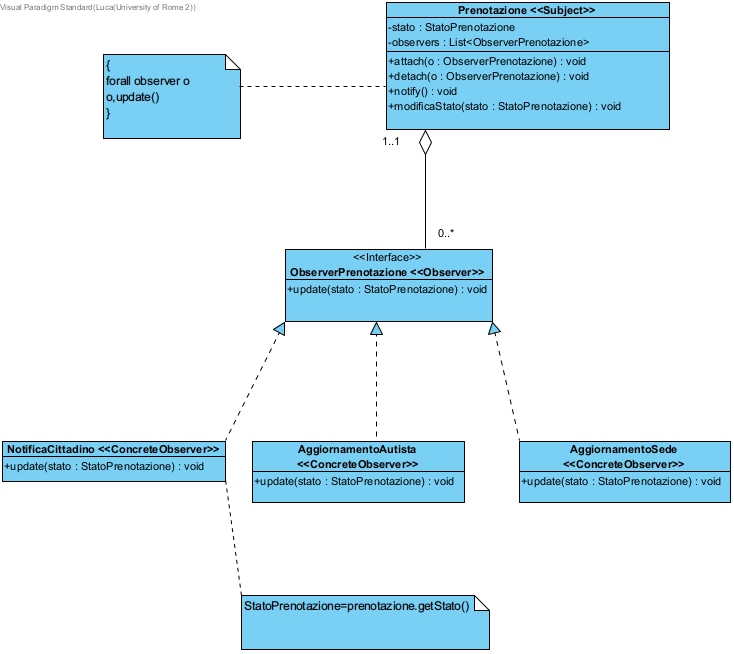
\includegraphics[width=0.95\textwidth]{figure/pattern_observer.jpg}
    \caption{Struttura UML del Design Pattern Observer applicato a MyAma}
    \label{fig:pattern_observer}
\end{figure}

% =========================================================================
% 6.3 STRATEGY PATTERN
% =========================================================================
\subsection{Strategy Pattern (Pattern Comportamentale)}

\subsubsection{Descrizione del Problema e Criticità di Design}
La gestione operativa dei ritiri a domicilio e la composizione dell'itinerario dei veicoli AMA sono processi complessi che variano a seconda delle condizioni quotidiane, delle politiche aziendali e delle disponibilità di mezzi e personale. In particolare, il sistema supporta differenti algoritmi di assegnazione:
\begin{itemize}[leftmargin=*]
    \item \textbf{Politica di Massimizzazione del Carico (\texttt{AssegnazionePerCapacita}):} algoritmo mirato a ottimizzare il riempimento (in volume e peso) dei mezzi prima del loro rientro in sede, minimizzando il numero complessivo di corse;
    \item \textbf{Politica di Prossimità Territoriale (\texttt{AssegnazionePerZona}):} algoritmo mirato a minimizzare i tempi e i chilometri percorsi, raggruppando i ritiri per aree limitrofe (stesso CAP).
\end{itemize}

Inserire la logica di tutti questi algoritmi direttamente all'interno del controllore di assegnazione, impiegando complesse e lunghe catene condizionali (\texttt{if-else} o \texttt{switch-case}), porterebbe alla creazione di una "God Class" difficilmente manutenibile (violazione del \textit{Single Responsibility Principle}). Inoltre, l'aggiunta di una futura nuova politica di smistamento richiederebbe la modifica di codice già testato e consolidato.

\subsubsection{Soluzione Progettuale e Vantaggi Architetturali}
Al fine di garantire flessibilità e manutenibilità, si è optato per l'applicazione dello \textbf{Strategy Pattern}. Questo pattern permette di incapsulare una famiglia di algoritmi all'interno di classi separate e intercambiabili a tempo di esecuzione, rendendo l'algoritmo indipendente dal client che ne fa uso.
Il controller dedicato alla pianificazione interagirà unicamente con un'interfaccia comune, delegando a runtime il calcolo dell'itinerario all'algoritmo (strategia) attualmente selezionato dall'amministratore di sede o dal sistema.

\subsubsection{Partecipanti}
\begin{itemize}[leftmargin=*]
    \item \textbf{Context:} la classe di controllo (\texttt{GestoreAssegnazione} / \texttt{PrenotazioneControl}). Essa mantiene un riferimento all'interfaccia \texttt{StrategiaAssegnazione} ed espone le operazioni per coordinare l'allocazione delle risorse delegando alla strategia attiva.
    \item \textbf{Strategy:} l'interfaccia \texttt{StrategiaAssegnazione} che dichiara il metodo astratto polimorfico \texttt{assegna(ritiro: RitiroDomicilio): Assegnazione}.
    \item \textbf{ConcreteStrategy:} le classi concrete che incapsulano le singole logiche aziendali, ovvero \texttt{AssegnazionePerCapacita} e \texttt{AssegnazionePerZona}. Ciascuna di esse implementa in modo differente il metodo dell'interfaccia.
\end{itemize}

\begin{figure}[H]
    \centering
    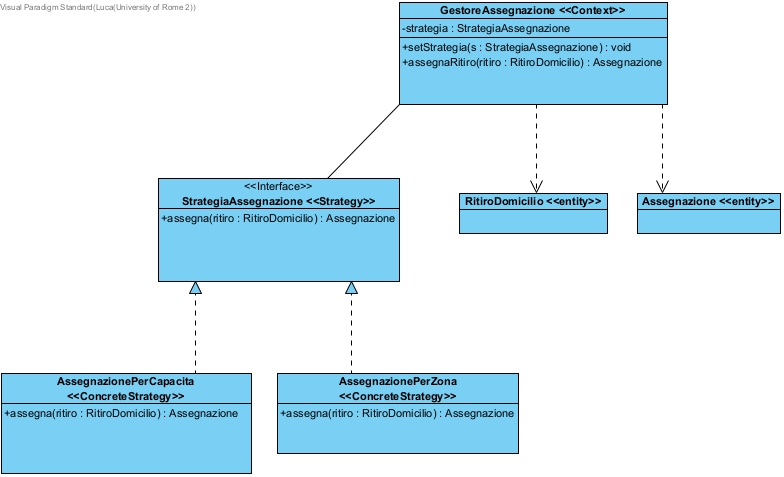
\includegraphics[width=0.95\textwidth]{figure/pattern_strategy.jpg}
    \caption{Struttura UML del Design Pattern Strategy per l'allocazione delle risorse}
    \label{fig:pattern_strategy}
\end{figure}
